%!TEX root = paper.tex"`

\section{Background}\label{sec:background}

\begin{figure}
\centering
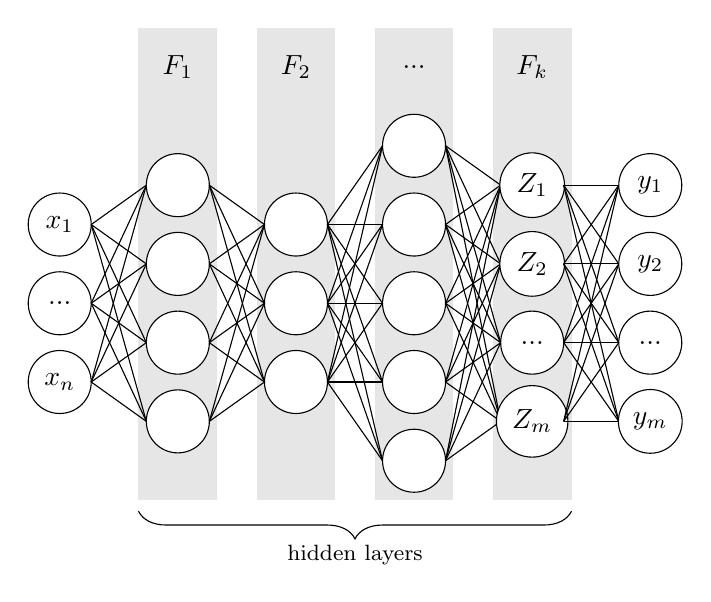
\begin{tikzpicture}[yscale=-1]
\tikzset{neuron/.style={
    shape=circle,
    fill=white,
    draw,
    minimum size=0.8cm
}}

%\draw[step=1cm,gray,very thin,fill=white] (0,0) grid (8,6);

\fill[opacity=0.2,fill=gray] (1,-0.5) rectangle (2,5.5);

\fill[opacity=0.2,fill=gray] (2.5,-0.5) rectangle (3.5,5.5);

\fill[opacity=0.2,fill=gray] (4,-0.5) rectangle (5,5.5);

\fill[opacity=0.2,fill=gray] (5.5,-0.5) rectangle (6.5,5.5);

\node[neuron] at (0, 2) {$x_1$};
\node[neuron] at (0, 3) {...};
\node[neuron] at (0, 4) {$x_n$};

\foreach \x in {1,...,3}{
	\draw (0.4, \x+1) -- (1.1,1.5);	\draw (0.4, \x+1) -- (1.1,2.5);
	\draw (0.4, \x+1) -- (1.1,3.5);
	\draw (0.4, \x+1) -- (1.1,4.5);
}

\node[] at (1.5, 0) {$F_1$};
\foreach \x in {2,...,5}{
	\node[neuron] at (1.5, \x-0.5) {};
	\draw (1.9, \x-0.5) -- (2.6,2);
	\draw (1.9, \x-0.5) -- (2.6,3);
	\draw (1.9, \x-0.5) -- (2.6,4);
}

\node[] at (3, 0) {$F_2$};
\foreach \x in {2,...,4}{
	\node[neuron] at (3, \x) {};
	\draw (3.4, \x) -- (4.1,1);	\draw (3.4, \x) -- (4.1,2);
	\draw (3.4, \x) -- (4.1,3);
	\draw (3.4, \x) -- (4.1,4);
	\draw (3.4, \x) -- (4.1,5);
}

\node[] at (4.5, 0) {...};
\foreach \x in {1,...,5}{
	\node[neuron] at (4.5, \x) {};
	\draw (4.9, \x) -- (5.6,1.5);	\draw (4.9, \x) -- (5.6,2.5);
	\draw (4.9, \x) -- (5.6,3.5);
	\draw (4.9, \x) -- (5.6,4.5);
}

\draw [decorate,decoration={brace,amplitude=10pt,mirror,raise=4pt},yshift=0pt]
(1,5.5) -- (6.5,5.5) node [black,midway,yshift=-0.7cm] {\footnotesize hidden layers};

\node[] at (6, 0) {$F_k$};
\foreach \x in {1,...,2}:
	\node[neuron] at (6, \x+0.5) {$Z_\x$};
\node[neuron] at (6, 3.5) {...};
\node[neuron] at (6, 4.5) {$Z_m$};

\foreach \x in {1,...,4}{
	\draw (6.4, \x + 0.5) -- (7.1,1.5);
	\draw (6.4, \x + 0.5) -- (7.1,2.5);
	\draw (6.4, \x + 0.5) -- (7.1,3.5);
	\draw (6.4, \x + 0.5) -- (7.1,4.5);
}

\foreach \x in {1,...,2}:
	\node[neuron] at (7.5, \x+0.5) {$y_\x$};
\node[neuron] at (7.5, 3.5) {...};
\node[neuron] at (7.5, 4.5) {$y_m$};
\end{tikzpicture}
\caption{Visualization of a neural network}
\label{fig:neuralnetwork}
\end{figure}

This section provides the general background knowledge required to understand the remainder of this paper.
In addition, the basic notation which is going to be used later is defined.
A reader familiar with the domain of adversarial machine learning is suggested to continue reading at Subsection~\ref{sec:threatmodel}.

\subsection{Deep Neural Networks}\label{subsec:dnn}
Deep neural networks (DNNs) are a form of machine learning algorithms based on a concept loosely analogous to the human brain.
On a conceptual level, DNNs take a vector of numbers as an input and assign it a output vector which represents the probability for each class which has been considered during training.
Thus, real-world input objects need to be transformed to a so called \enquote{feature space}, their mathematical abstraction that can be passed to the DNN.
In the context of image recognition, this relates to taking each input pixel's color channel as an input feature.
Having a look on the inner structure, neural networks consist of a set of nodes (\enquote{neurons}), which are organized in successive layers.
Each neuron is represented by a mathematical function taking a weighted sum of inputs and returning the value of a previously specified activation function.
Currently, the sigmoid function $H : x \mapsto \frac{1}{1 + e^{-x}}$ and the rectified linear unit (ReLU) function $H : x \mapsto max(0, x)$ are the most common activation functions in practice.
In a fully connected architecture, the activation of each neuron is affected by each output of the previous layer.
More precisely, each neuron's output is defined as the weighted sum of all previous layer's outputs, subsequently transformed by an activation function.
The output of the final layer is transformed using a softmax function $\sigma : x \mapsto \frac{e^{x_i}}{\sum_{j=1}^{N} e^{x_j}}$ for $\forall i \in N$ with $N$ as the number of dimensions.
Simply put, this function returns a confidence score by mapping each value to the range $(0, 1]$ and scaling the output such that the sum of all outputs is equal to one.
This is the previously mentioned output probability assigned to a certain input.
The quality of a DNN's classification is determined by a loss function, which indicates the distance of a given output from the optimal solution.

Before a network can be used, it needs to be trained.
The training phase includes repeatedly feeding given input-output pairs through the network, evaluating the output using the loss function and adjusting the weights.
For the latter, a backpropagation algorithm is used which decreases the weights of previous layers that contributed most to the loss, effectively increasing the relative impact of those weights contributing to a correct classification.
At the beginning, the weights are usually random and after multiple training iterations (epochs), the network starts to infer a functional dependency from the training samples.
The set of learned weights is referred to as a model $\theta$.
Furthermore, there are parameters that are not directly related to the learned model but affect the learning process.
These are referred to as \enquote{hyperparameters}.
Two examples for such a hyperparameter are the learning rate and the selected optimizer.

Additionally, Convolutional Neural Networks (CNNs) are going to be examined in the course of this project.
They are an extension of regular DNNs and have proven to work well in the domain of image classification \cite{matsugu2003subject, krizhevsky2012imagenet}.
The key difference here is that there are additional types of layers.
Convolution layers perform a special operation taking a spatial sliding window (called \enquote{receptive field} or \enquote{filter}) and returning its activation.
Depending on the architecture, multiple filters may be used.
After the convolution layer, a pooling layer reduces the dimensionality using a specified downsampling function.
For example, the \enquote{Max Pooling} returns the maximum value in a spatial neighborhood.
As a result, the CNN is able to recognize edges and other spatial characteristics of an image without any preprocessing.

\subsection{Distance Metrics}\label{subsec:metrics}
The definition of distances in a feature space is crucial for a successful classification.
In the domain of image recognition, it quantifies how different two images are.
Selecting an appropriate distance metric is relevant when perturbing an image because each attack algorithm is optimized under a certain metric.
Evaluating the suitability of a given metric in this context however is not trivial, because it depends more on how humans perceive images than on how big their differences are in theory.
An attack might yield good results according to a specific metric while a human observer would disagree on this.
To give a basic notion of distance metrics, the three most commonly used metrics are briefly presented below.

The $L_0$ distance between two images counts how many pixels are different from each other.
Using this metric is based on the simple idea that images look more different the more pixels have been altered.
An example of an attack that uses this metric is the Jacobian-based Saliency Map Attack \cite{papernot2016limitations}.
In contrast to that, the $L_\infty$ norm measures the maximum difference of any pixel.
This metric reflects the situation in which single strongly modified pixels are immediately recognizable.
For instance, the Fast-Gradient Sign Method is optimized under this distance metric~\cite{szegedy2015explaining}.
Finally, there is the $L_2$ norm which appears to be the most beneficial when creating adversarial examples.
It computes the square root of the pixel-wise squared sum of differences of two images.
This is equivalent to a distance in euclidean space which gives a natural sense of the dissimilarity between two images.

\subsection{Notation}\label{subsec:notation}
In the remainder of this document, different aspects related to Machine Learning are going to be analyzed and discussed.
The utilized notation is briefly presented in this subsection.

%TODO define only notation that is actually used
% perturbed image's distance delta
% norm, L2-norm